\section{moeo\-Hypervolume\-Binary\-Metric$<$ Objective\-Vector $>$ Class Template Reference}
\label{classmoeoHypervolumeBinaryMetric}\index{moeoHypervolumeBinaryMetric@{moeoHypervolumeBinaryMetric}}
Hypervolume binary metric allowing to compare two objective vectors as proposed in Zitzler E., K\~{A}�nzli S.  


{\tt \#include $<$moeo\-Hypervolume\-Binary\-Metric.h$>$}

Inheritance diagram for moeo\-Hypervolume\-Binary\-Metric$<$ Objective\-Vector $>$::\begin{figure}[H]
\begin{center}
\leavevmode
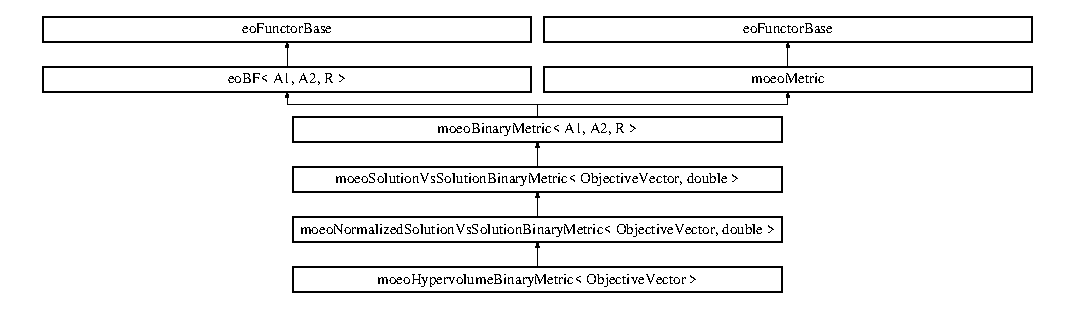
\includegraphics[height=3.70044cm]{classmoeoHypervolumeBinaryMetric}
\end{center}
\end{figure}
\subsection*{Public Member Functions}
\begin{CompactItemize}
\item 
\bf{moeo\-Hypervolume\-Binary\-Metric} (double \_\-rho=1.1)
\begin{CompactList}\small\item\em Ctor. \item\end{CompactList}\item 
double \bf{operator()} (const Objective\-Vector \&\_\-o1, const Objective\-Vector \&\_\-o2)
\begin{CompactList}\small\item\em Returns the volume of the space that is dominated by \_\-o2 but not by \_\-o1 with respect to a reference point computed using rho. \item\end{CompactList}\end{CompactItemize}
\subsection*{Private Member Functions}
\begin{CompactItemize}
\item 
double \bf{hypervolume} (const Objective\-Vector \&\_\-o1, const Objective\-Vector \&\_\-o2, const unsigned int \_\-obj, const bool \_\-flag=false)
\begin{CompactList}\small\item\em Returns the volume of the space that is dominated by \_\-o2 but not by \_\-o1 with respect to a reference point computed using rho for the objective \_\-obj. \item\end{CompactList}\end{CompactItemize}
\subsection*{Private Attributes}
\begin{CompactItemize}
\item 
double \bf{rho}\label{classmoeoHypervolumeBinaryMetric_2498b6010719249121e3a371978d927b}

\begin{CompactList}\small\item\em value used to compute the reference point from the worst values for each objective \item\end{CompactList}\item 
\bf{moeo\-Pareto\-Objective\-Vector\-Comparator}$<$ Objective\-Vector $>$ \bf{pareto\-Comparator}\label{classmoeoHypervolumeBinaryMetric_2bbeb34a5bfde25b9eadc7eca899906e}

\begin{CompactList}\small\item\em Functor to compare two objective vectors according to Pareto dominance relation. \item\end{CompactList}\end{CompactItemize}


\subsection{Detailed Description}
\subsubsection*{template$<$class Objective\-Vector$>$ class moeo\-Hypervolume\-Binary\-Metric$<$ Objective\-Vector $>$}

Hypervolume binary metric allowing to compare two objective vectors as proposed in Zitzler E., K\~{A}�nzli S. 

: Indicator-Based Selection in Multiobjective Search. In Parallel Problem Solving from Nature (PPSN VIII). Lecture Notes in Computer Science 3242, Springer, Birmingham, UK pp.832\^{a}��842 (2004). This indicator is based on the hypervolume concept introduced in Zitzler, E., Thiele, L.: Multiobjective Optimization Using Evolutionary Algorithms - A Comparative Case Study. Parallel Problem Solving from Nature (PPSN-V), pp.292-301 (1998). 



Definition at line 29 of file moeo\-Hypervolume\-Binary\-Metric.h.

\subsection{Constructor \& Destructor Documentation}
\index{moeoHypervolumeBinaryMetric@{moeo\-Hypervolume\-Binary\-Metric}!moeoHypervolumeBinaryMetric@{moeoHypervolumeBinaryMetric}}
\index{moeoHypervolumeBinaryMetric@{moeoHypervolumeBinaryMetric}!moeoHypervolumeBinaryMetric@{moeo\-Hypervolume\-Binary\-Metric}}
\subsubsection{\setlength{\rightskip}{0pt plus 5cm}template$<$class Objective\-Vector$>$ \bf{moeo\-Hypervolume\-Binary\-Metric}$<$ Objective\-Vector $>$::\bf{moeo\-Hypervolume\-Binary\-Metric} (double {\em \_\-rho} = {\tt 1.1})\hspace{0.3cm}{\tt  [inline]}}\label{classmoeoHypervolumeBinaryMetric_01a07711a7c9f38cdc2c76e40a3c5958}


Ctor. 

\begin{Desc}
\item[Parameters:]
\begin{description}
\item[{\em \_\-rho}]value used to compute the reference point from the worst values for each objective (default : 1.1) \end{description}
\end{Desc}


Definition at line 37 of file moeo\-Hypervolume\-Binary\-Metric.h.

References moeo\-Hypervolume\-Binary\-Metric$<$ Objective\-Vector $>$::rho.

\subsection{Member Function Documentation}
\index{moeoHypervolumeBinaryMetric@{moeo\-Hypervolume\-Binary\-Metric}!operator()@{operator()}}
\index{operator()@{operator()}!moeoHypervolumeBinaryMetric@{moeo\-Hypervolume\-Binary\-Metric}}
\subsubsection{\setlength{\rightskip}{0pt plus 5cm}template$<$class Objective\-Vector$>$ double \bf{moeo\-Hypervolume\-Binary\-Metric}$<$ Objective\-Vector $>$::operator() (const Objective\-Vector \& {\em \_\-o1}, const Objective\-Vector \& {\em \_\-o2})\hspace{0.3cm}{\tt  [inline]}}\label{classmoeoHypervolumeBinaryMetric_c147309a5ba6b365be926e6083c5b9f2}


Returns the volume of the space that is dominated by \_\-o2 but not by \_\-o1 with respect to a reference point computed using rho. 

\begin{Desc}
\item[Warning:]don't forget to set the bounds for every objective before the call of this function \end{Desc}
\begin{Desc}
\item[Parameters:]
\begin{description}
\item[{\em \_\-o1}]the first objective vector \item[{\em \_\-o2}]the second objective vector \end{description}
\end{Desc}


Definition at line 63 of file moeo\-Hypervolume\-Binary\-Metric.h.

References moeo\-Hypervolume\-Binary\-Metric$<$ Objective\-Vector $>$::hypervolume(), and moeo\-Hypervolume\-Binary\-Metric$<$ Objective\-Vector $>$::pareto\-Comparator.\index{moeoHypervolumeBinaryMetric@{moeo\-Hypervolume\-Binary\-Metric}!hypervolume@{hypervolume}}
\index{hypervolume@{hypervolume}!moeoHypervolumeBinaryMetric@{moeo\-Hypervolume\-Binary\-Metric}}
\subsubsection{\setlength{\rightskip}{0pt plus 5cm}template$<$class Objective\-Vector$>$ double \bf{moeo\-Hypervolume\-Binary\-Metric}$<$ Objective\-Vector $>$::hypervolume (const Objective\-Vector \& {\em \_\-o1}, const Objective\-Vector \& {\em \_\-o2}, const unsigned int {\em \_\-obj}, const bool {\em \_\-flag} = {\tt false})\hspace{0.3cm}{\tt  [inline, private]}}\label{classmoeoHypervolumeBinaryMetric_e841d13001c63b043981a41fcb49218a}


Returns the volume of the space that is dominated by \_\-o2 but not by \_\-o1 with respect to a reference point computed using rho for the objective \_\-obj. 

\begin{Desc}
\item[Parameters:]
\begin{description}
\item[{\em \_\-o1}]the first objective vector \item[{\em \_\-o2}]the second objective vector \item[{\em \_\-obj}]the objective index \item[{\em \_\-flag}]used for iteration, if \_\-flag=true \_\-o2 is not talen into account (default : false) \end{description}
\end{Desc}


Definition at line 96 of file moeo\-Hypervolume\-Binary\-Metric.h.

References moeo\-Normalized\-Solution\-Vs\-Solution\-Binary\-Metric$<$ Objective\-Vector, double $>$::bounds, and moeo\-Hypervolume\-Binary\-Metric$<$ Objective\-Vector $>$::rho.

Referenced by moeo\-Hypervolume\-Binary\-Metric$<$ Objective\-Vector $>$::operator()().

The documentation for this class was generated from the following file:\begin{CompactItemize}
\item 
moeo\-Hypervolume\-Binary\-Metric.h\end{CompactItemize}
